\documentclass{beamer}

\usepackage{
    hyperref,
    multicol,
    soul,
    minted,
    xcolor,
    subfig,
    wrapfig,
    standalone,
    tikz,
}
\definecolor{LightGray}{gray}{0.9}
\setbeamercovered{transparent}
\setbeameroption{show notes on second screen=right}
% \setbeameroption{hide notes}
\graphicspath{{figures}}

\setlength{\columnsep}{0mm}

\title{A Simple Parcel Theory Model of Downdrafts in Atmospheric Convection}
\author{
    Thomas Schanzer
    \texorpdfstring{\\}{}
    \small \texorpdfstring{
        \url{https://github.com/tschanzer/taste-of-research-21T3}}{
        https://github.com/tschanzer/taste-of-research-21T3
    }
    \texorpdfstring{\\ \vspace{5mm}}{}
    Supervisor: Prof. Steven Sherwood}
\institute{UNSW School of Physics}
\date{Thursday 25 November 2021}

\begin{document}

\frame{\titlepage}
\note[itemize]{
    \item Present a simple model...
    \item Firstly: thank Steve for his patient guidance
    \item Thank group for opportunity to speak
}

\begin{frame}
    \frametitle{Aim and Motivation}
    \note<1>[item]{
        Downdrafts play an important role
        (mass, momentum, heat and moisture)
    }

    \begin{columns}
    \begin{column}{0.5\textwidth}
        \vspace{3mm}

        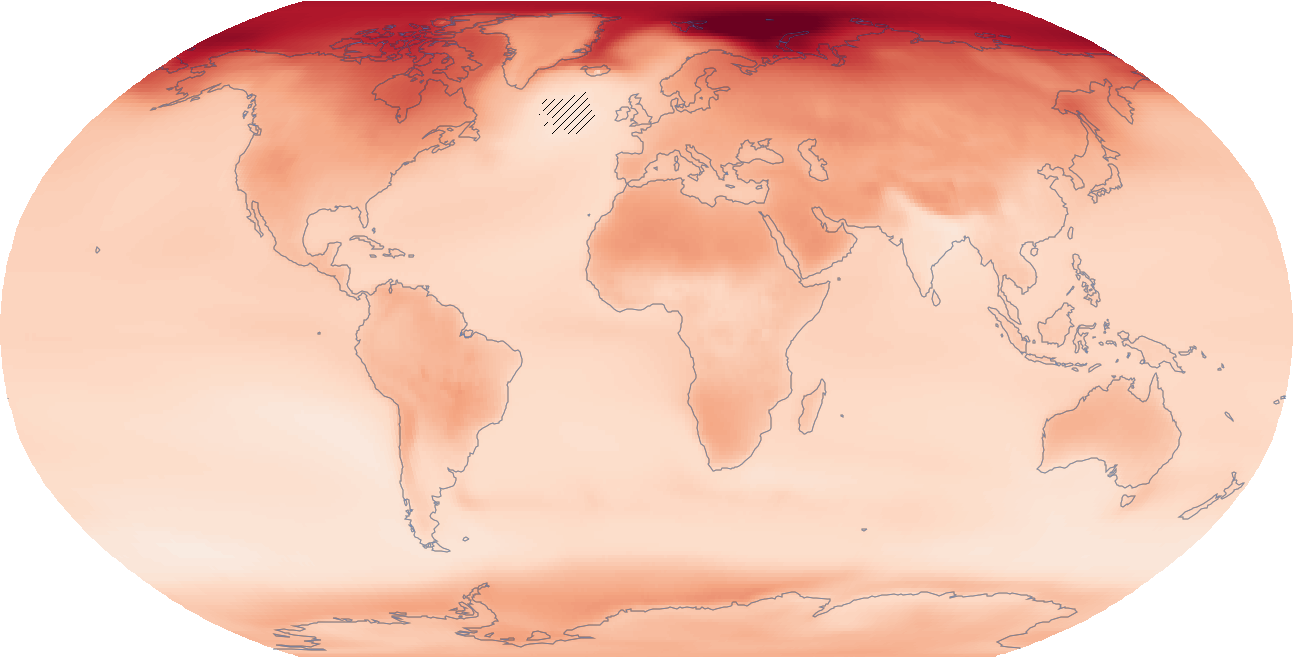
\includegraphics[height=2.5cm]{figures/ipcc_model_temp_cropped.png}
        \centering \footnotesize
        {\color{blue} (a)} Convection parametrisation in global climate models
    \end{column}
    \begin{column}{0.5\textwidth}
        \hspace{-7mm}%
        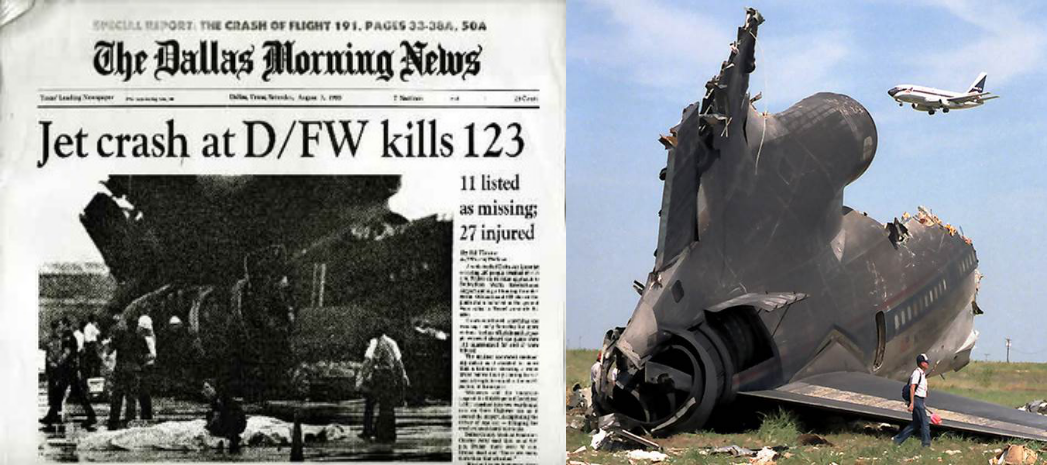
\includegraphics[height=2.5cm]{figures/delta191_side.png}

        \hspace{-11mm}%
        \centering \footnotesize
        {\color{blue} (b)} Forecasting dangerous microbursts
    \end{column}
    \end{columns}

    \begin{center}
        \tiny \color{gray} (a): IPCC AR6 interactive atlas.
        (b): US National Weather Service.
    \end{center}
    \note<1>[item]{
        Intergovernmental Panel on Climate Change \#6, average temperature
        increase across 34 global climate models
    }
    \note<1>[item]{
        Delta Flight 191, Dallas/Fort Worth 1985 (one of several)
    }

    \pause
    \begin{block}{Question}
        Which processes and conditions initiate, and which
        maintain or inhibit, downdrafts?
    \end{block}
    \vspace{5mm}
    \note<2>[item]{Both prompt us to ask...}
\end{frame}

\begin{frame}
    \frametitle{Literature}
    \emph{Knupp and Cotton (1985)}
    \footnote{ \tiny
        Knupp, KR \& Cotton, WR 1985, ‘Convective cloud downdraft
        structure: An interpretive survey’, Reviews of geophysics (1985),
        vol. 23, no. 2, pp. 183–215.}
    identify four downdraft types:
    \vspace{-2mm}
    \begin{multicols}{2}
        \small
        \begin{itemize}
            \item Precipitation-associated (PR)
            \item Penetrative (P)
            \item Cloud-edge (E)
            \item Overshooting (O)
        \end{itemize}
    \end{multicols}
    \vspace{-3mm}
    \begin{figure}[ht]
        \centering
        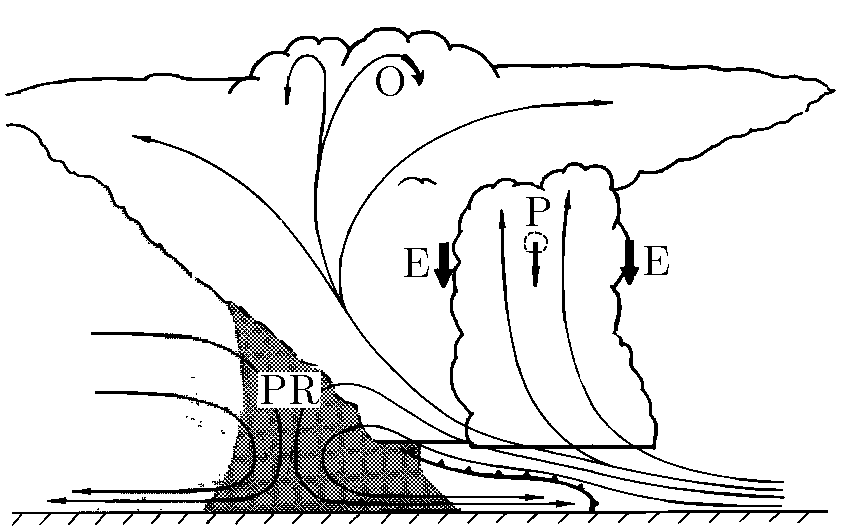
\includegraphics[width=0.6\linewidth]{figures/knupp_cotton_types.pdf}
    \end{figure}
    \vspace{-3mm}
    \centering \tiny Adapted from \emph{Knupp and Cotton (1985)}.

    \note[item]{
        Four qualitative answers identified in literature...
    }
    \note[item]{
        This work: primarily PR, but model is general -- applicable to
        provided appropriate initial conditions
    }
\end{frame}

\begin{frame}
    \frametitle{Background: Parcel Theory}
    \note<1>[item]{The basis of the model is...}

    \uncover<1>{
    \begin{itemize}
        \item Vertical motion under buoyant forces only:
            \[b
            = \frac{
                \rho_\text{env} - \rho_\text{parcel}
            }{
                \rho_\text{parcel}
            }g.\]
        \item Descent is (dry or moist) adiabatic
    \end{itemize}
    }
\end{frame}

\begin{frame}[fragile]
    \frametitle{Methods}
    \begin{columns}
    \begin{column}{0.7\textwidth}
    \vfil
    \note<1>[item]{
        From scratch in Python, using parcel theory as basis,
        theoretical foundation
    }
    \note<1>[item]{
        Buoyancy: need to know temperature vs. height
    }

    \uncover<1>{%
    \textbf{Goal:} calculate parcel temperature $\to$ density as
    functions of height
    }

    \vspace{3mm}
    \uncover<2>{%
    \textbf{Complication:} \emph{entrainment}
    }
    \note<2>[item]{Not covered by traditional parcel theory}
    \note<2>[item]{
        Relative amount dictated by entrainment rate (constant, linear)
    }
    \note<2>[item]{Explain phase equilibration, competing factors}


    \vspace{3mm}
    \uncover<3>{%
    Supply \emph{any} environmental temperature and moisture profile
    }
    \note<3>[item]{
        Need to know... (both for entrainment and buoyancy),
        Important capability: ..., (more later)
    }
    \note<3>[item]{
        Real or idealised (used idealised, explain, constant
        relative humidity above boundary layer)
    }

    \vspace{3mm}
    \uncover<4>{%
    Choose initial conditions and numerically solve
    \[\frac{d^2 z}{dt^2} = b(z).\]
    }
    \note<4>{
        Now relatively simple (most work: finding $b(z)$)
    }

    \vfil
    \end{column}
    \begin{column}{0.3\textwidth}
        \begin{overlayarea}{\textwidth}{7cm}
        \only<2>{
        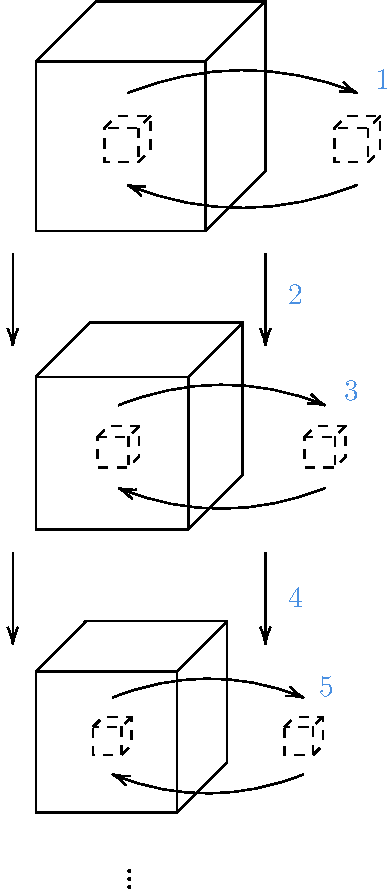
\includegraphics[width=\linewidth]{entraining_descent.pdf}
        }
        \only<3>{

        \vspace{5mm}
        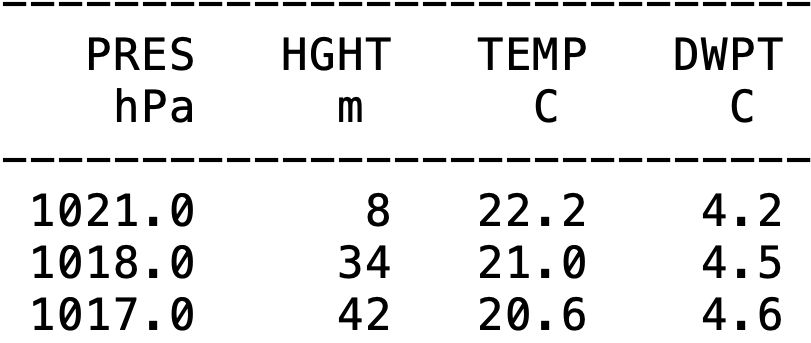
\includegraphics[width=\linewidth]{sounding.png}

        \vspace{1cm}
        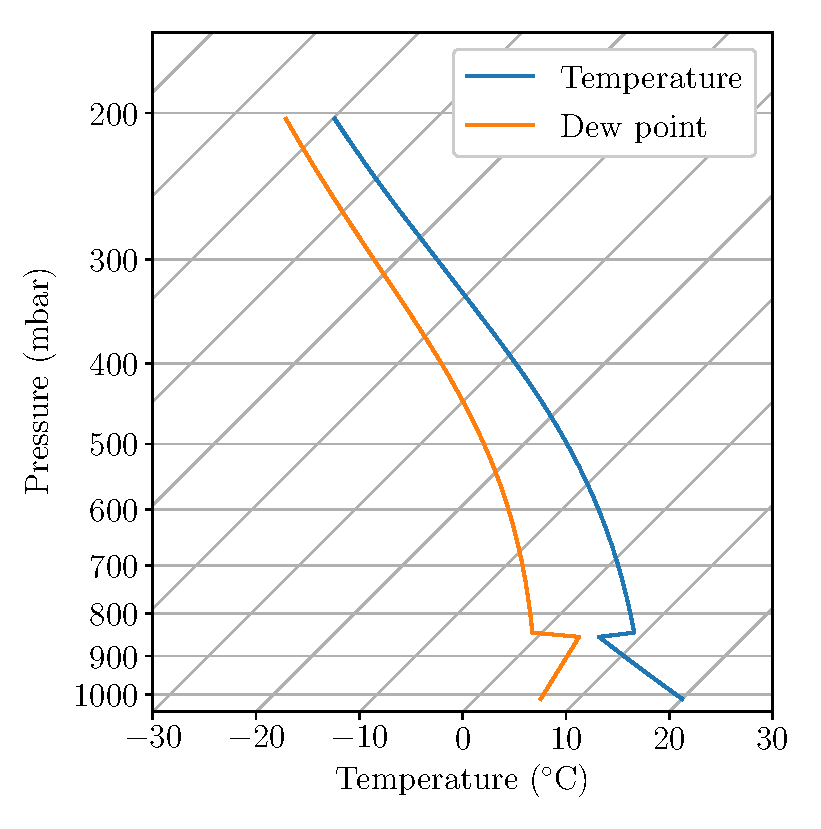
\includegraphics[width=\linewidth]{skewt.eps}
        }
        \end{overlayarea}
    \end{column}
    \end{columns}
\end{frame}

\begin{frame}
    \frametitle{Results: Precipitation Enhances Downdrafts}
    \begin{figure}[ht]
        \centering
        \includegraphics[width=0.9\linewidth]%
            {figures/motion_vs_initial_conditions_50RH_1perkm.eps}
    \end{figure}
    \note[item]{Imagine...}
    \note[item]{
        Bottom row: explain horizontal axis
    }
    \note[item]{Explain: why? (condensate loading, moist descent)}
\end{frame}

\begin{frame}
    \frametitle{Results: Entrainment Inhibits Downdrafts}
    \begin{figure}[ht]
        \centering
        \includegraphics[width=0.9\linewidth]%
            {figures/motion_vs_entr_rate_2gram_50RH.eps}
    \end{figure}
    \note[item]{
        Similar to before, fix initial conditions: saturation, 2 g/kg
        liquid
    }
    \note[item]{Explain entrainment rate (legend)}
    \note[item]{Why?}
\end{frame}

\begin{frame}
    \frametitle{Results: Atmospheric Dryness Enhances Downdrafts}
    \begin{figure}[ht]
        \centering
        \includegraphics[width=0.9\linewidth]%
            {figures/motion_vs_RH_2gram_1perkm.eps}
    \end{figure}
    \note[item]{
        Idealised profiles... vary humidity (constant above boundary
        layer)
    }
    \note[item]{
        Otherwise: initial conditions, entrainment rate constant
    }
    \note[item]{Why?}
\end{frame}

\begin{frame}
    \frametitle{Results: DCAPE and DCIN}
    \footnotesize
    \[
        \text{DCAPE}
        = \int_\text{surface}^\text{min $T_W$}
        \max \{ b^*(z), 0 \} ~\text{d}z
        \qquad
        \text{DCIN}
        = \int_\text{surface}^\text{min $T_W$}
        \min \{ b^*(z), 0 \} ~\text{d}z
    \]
    \only<1>{
    \begin{columns}
    \begin{column}{0.1\textwidth}
    \end{column}
    \begin{column}{0.35\textwidth}
        \small
        \begin{itemize}
            \item No entrainment
            \item Moist descent only
            \item Pseudoadiabatic
        \end{itemize}
    \end{column}
    \begin{column}{0.4\textwidth}
        \small
        \begin{itemize}
            \item Fixed integration limits
            \item Fixed initial conditions
        \end{itemize}
    \end{column}
    \begin{column}{0.15\textwidth}
    \end{column}
    \end{columns}
    \note<1>[item]{Thanks to Tim}
    \note<1>[item]{DCAPE and DCIN measure...}
    \note<1>[item]{Definitions}
    \note<1>[item]{
        Just a fancy overcomplicated way of finding DCAPE?
        According to the conventional definitions...
    }

    }
    \visible<2>{
    \begin{figure}[ht]
        \centering
        \includegraphics[width=0.65\linewidth]%
            {figures/strength_vs_dcape_dcin_2gram_1perkm.pdf}
    \end{figure}
    }
    \note<2>{Relate to previous plots}
\end{frame}

\begin{frame}
    \frametitle{Conclusions}

    \uncover<1>{%
    \textbf{Conclusions:} downdraft strength and penetration are
    \begin{itemize}
        \item Increased by precipitation evaporation and condensate loading,
        \item Reduced by entrainment of environmental air,
        \item Increased by atmospheric dryness,
        \item Strongly linked to DCAPE and DCIN.
    \end{itemize}
    }
    \note<1>{To summarise...}
\end{frame}
\begin{frame}
    \frametitle{Next Steps}
    \begin{columns}
    \begin{column}{0.5\textwidth}
        \uncover<1>{%
        \textbf{Application:} supplement basic sounding analysis methods used
        in weather forecasting
        }
        \note<1>[item]{
            Mentioned earlier: any profile of environmental temperature, moisture
            (needed for...)
        }
        \note<1>[item]{
            Measured 2x/day all over the world, forecasters calculate indices...
        }
        \note<1>[item]{
            Sydney: assess downdraft potential without time, effort, expense...
        }
    \end{column}
    \begin{column}{0.5\textwidth}
        \visible<1>{
        \centering
        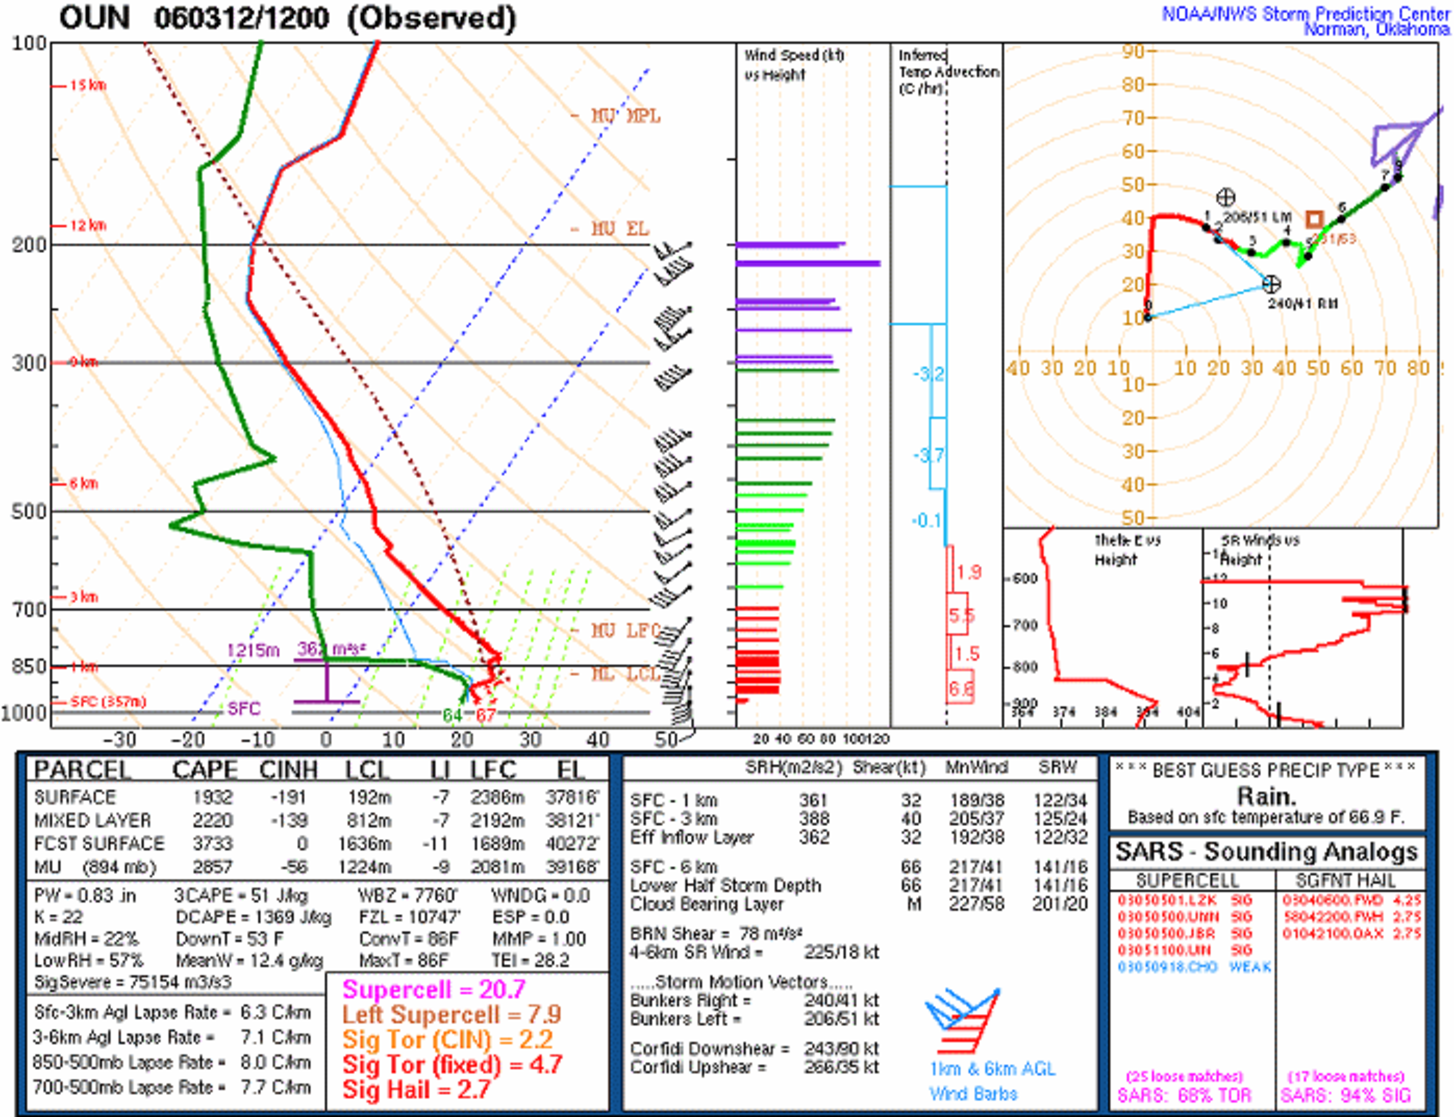
\includegraphics[width=\linewidth]{figures/sounding_analysis.pdf}
        \tiny Source: NOAA Storm Prediction Center
        }
    \end{column}
    \end{columns}

    \uncover<2>{%
    \textbf{Future Work:}
    \begin{itemize}
        \item Consider other forces, e.g. drag
        \item Model more advanced dynamics, e.g. entrainment from
            updrafts
        \item Support the findings of more advanced models
    \end{itemize}
    }
    \note<2>[item]{
        Model is simple, with a few improvements: accurate numerical
        predictions... (mention momentum)
    }
    \note<2>[item]{
        Steve + colleague at the Max Planck
        Institute for Meteorology, machine learning
    }
    \note<2>[item]{Thank again}
\end{frame}
\end{document}